%allowed options finnish, swedish, english
%after changing the language you may be forced to use recompile from scratch to get rid of errors
\documentclass[english]{tktltiki}
\usepackage{epsfig}
\usepackage{graphicx,subfigure}
\usepackage{url}
\usepackage{lipsum}

\begin{document}
%\doublespacing
\onehalfspacing
%\singlespacing

\title{Testing and Verification of RESTful Web Services}
\author{Ege Can Özer}
\date{\today}

\maketitle
\numberofpagesinformation{\numberofpages\ pages + \numberofappendixpages\ appendices}

\classification{\protect{\ \\
		\  Applied computing $\rightarrow$ Enterprise computing  $\rightarrow$ Service-oriented architectures\
}}


\keywords{Service-oriented architectures, Software testing, Web services, REST}

\begin{abstract}
\setlength{\parindent}{1cm} % Default is 15pt.
\setlength{\leftskip}{1cm}
%\hangindent=1cm
Today, service-oriented architectures (SOA) are widely used and have become a major discipline for enterprise applications. Until the last decade, the most popular way to implement the services was using Simple Object Access Protocol (SOAP). Including the big companies such as Google, Facebook, Twitter, the direction moved towards to Representational State Transfer (REST) services due to the advantages such as its lightweight and scalability.

%Software testing is important and crucial in any software development process, because of error handling, quality assurance,  and performance awareness. 
Unlike the conventional software testing, web services require different testing methods due to their loosely coupled, headless, and distributed architectures. In the literature, general trends and challenges of SOA testing reviewed, but the discussion primarily focused on the SOAP web services. Having said that there is a demand to demonstrate recent approaches concerning testing RESTful services.

This paper presents different means for testing and verification of RESTful web services, showing the advantages and disadvantages of testing tools and current approaches; and includes an analysis of five of this specialized methods from the service testing point of view. Based on the comparative results, we will identify issues for the future work.
\\
\end{abstract}

\mytableofcontents

\section{Introduction}
Today, service-oriented architectures (SOA) are widely used and have become a major discipline for enterprise applications. Until the last decade, the most popular way to implement the services was using Simple Object Access Protocol (SOAP). Including the big companies such as Google, Facebook, Twitter, the direction moved towards to Representational State Transfer (REST) services due to the advantages such as its lightweight and scalability. In 2012, ProgrammableWeb reported that 75\% out of all APIs follows REST architectural style, and it continues to grow exponentially \cite{programmableweb}.

Testing plays a critical role to ensure certain reliability and quality for SOAs. Unlike the conventional system-level testing, testing methods differ in service-centric systems. In the literature there are many articles presents several approaches to address the problems in SOA testing. Canfora and Di Penta \cite{canfora2009service} report a survey of SOA testing, they analyze the challenges from different stakeholders point of view and categorize them based on testing levels. Whereas, Bozkur et al. \cite{bozkurt2013testing} extends the research by surveying 177 papers, identifies the features of testing strategies. However, in both of the surveys, the discussion primarily focuses on SOAP services.

Nevertheless, many of the testing related issues in SOA based web-services are common and inherited by RESTful web-services. Testing challenges in web services emerge from distributedness, loose-coupling, and lack of reliability of WWW as a common communication framework \cite{chakrabarti2009test}. Moreover, headless (lack of graphical user interface) structure of the web services makes manual testing difficult to interpret. Many other challenges do also exist due to the complexity and the limitations that are imposed by the SOA environment \cite{canfora2006testing, canfora2009service, bozkurt2013testing}. Still, various strategies have been put forward to handle testing and validation of SOA, ranging from testing frameworks, model-based testing to evolutionary algorithms.

In this article, we present and give a brief analysis of five different testing approaches developed for RESTful services that are advanced during the last decade. First, Chakrabarti and Kumar \cite{chakrabarti2009test} introduce a testing framework that contributes to many novel techniques. Second, Chakrabarti and Rodriquez \cite{chakrabarti2010connectedness} demonstrate a particular feature of RESTful web-service testing, named \textit{connectedness}, which is an essential aspect for resource-oriented architectures to assure. In the third article Pinheiro et al. \cite{pinheiro2013model} present a model-based testing approach using UML protocol state machine to generate test cases automatically. Next article by Navas et al. \cite{navas2014rest} show an automatic error detection system based on statistical information without fully knowing its full-service specification. With that, they open an opportunity to apply Machine Learning algorithms to this area. The final article by Andrea Arcuri \cite{arcuri2017restful} propose an automated white-box testing approach, where test cases are generated using an evolutionary algorithm.

The rest of this document is organized as follows. In section 2, we survey the available different research around testing RESTful web-services. Hence, section 2 is structured in two blocks. The first block presents the overview of system description and principal features of these five methods. Then in the following block, we provide a comparative analysis. In section 3, we will propose ideas for future research in this area. The last section summarizes and concludes the paper.
%In the literature, general trends and challenges of SOA testing reviewed, but the discussion primarily focused on the SOAP web services \cite{canfora2009service, bozkurt2013testing}. Moreover, REST differs from others due to its architectural constraints, such as statelessness, cacheability, uniform interface. Having said that there is a demand to demonstrate recent approaches concerning testing RESTful services.

%On the other hand, Canfora and Di Penta \cite{canfora2009service, canfora2006testing} put forward several challenges and perspectives in the context of testing service-oriented systems, by which essentially fits in consideration of RESTful services. For example, adaptiveness is excellent and presents a strong relation to transparency problem of REST services. Further, Bozkurt et al. extend the testing perspectives each one separately, total of 14 groups; whereas Canfora and Di Penta consider only in 5 main groups. In an attempt to present recent studies about testing restful services, will follow studies as mentioned earlier as our direction.

\section{Testing methods for REST services}
%Challenges in testing RESTful systems.
As far as testing web-services are concerned much research has gone into investigating challenges stand in this area \cite{canfora2009service, bozkurt2013testing}. In particularly for RESTful web-services, the main challenges emerge from distributedness, loose-coupling, and lack of reliability of WWW as a common communication framework \cite{chakrabarti2009test}. 

Distributedness architecture of the services often minimizes the controllability and observability of the system, and it makes locating the failures difficult. Lack of transparency complicates and enforces an unsystematic manual test case generation by the service testers. So that, designed test cases are only error-prone to developer's opinion \cite{navas2014rest}. Likewise, headless (lack of GUI) architecture of the web-services poses the similar issue. Differently, loose-coupling makes the test case creation demanding because of data incompatibility between subsystems, especially if the working mechanism of the system is unknown. Extending the testing coverage by including other applications such as 3rd party web-services and databases makes it even more complicated to test RESTful web-services.

During the last years, there has been much progress related to testing RESTful web services. For example concerning the development of testing frameworks, \textit{Test-the-rest} \cite{chakrabarti2009test} demonstrated novel techniques to test RESTful services. Then following more specific approaches has undergone \cite{chakrabarti2010connectedness}, such as testing the \textit{connectedness} of the RESTful services. Subsequently, many of the approaches benefited from model-driven engineering methodology, Navas et al. \cite{navas2014rest} as an instance. As a result of recent advancements in the machine learning algorithms, new approaches \cite{navas2014rest, arcuri2017restful} have also been adapted to this field. Since it is not possible to cover every aspect of the RESTful web-service testing, which in general categorized in \cite{canfora2009service, bozkurt2013testing}, we are only going to focus on a small set of articles. Hence, the following section provides an overview of system description of the articles as mentioned earlier.

\subsection{System description and principal features}
% First article
\textbf{Test-the-rest: An approach to testing restful web-services \cite{chakrabarti2009test}.} The first article authored by Chakrabarti and Kumar \cite{chakrabarti2009test} presents a black-box testing framework called \textit{Test-the-rest (TTR)}. The testing framework carries the following features: the capability to do functional and non-functional testing, automatic test case generation, extensible architecture design for testing RESTful web-services, specialized test specification language that supports reusable and composable test cases.

TTR designed architecturally similar to WebInject \cite{webinject} tool as the idea of writing test cases based on external XML files supports the automatic test generation. The general architecture of TTR is shown in Figure \ref{fig:ttr_system}. According to this, first, the input test case has written go through a sanity check by the test case validator. Then HTTP engine issues the HTTP methods given under the test case. HTTP responses are validated for each test case by the external verifiers (e.g., XML validator plugin) and the test verdict is given. 

However, the main contribution is the test specification language. The test specification language is XML formatted and similar to WebInject's test case language and Web Application Description Language (WADL). It supports composite test case validation by making use of logical operators, test case composition by allowing reuse and nested testing. Parametrization is also supported so that test cases can be generated with an arbitrary input automatically. An example of test case given in Figure \ref{fig:ttr_test}.

Experiments took place in an internal infrastructure of authors'. In the first phase 300 manual test cases written by the testers, and tested daily where 5-10 test cases failed daily corresponding to real system bugs. In the second phase, test case generation is automatized and generated 42,767 test cases where the 38,016 test cases failed due to two significant bugs. After fixing the bugs, the number of failures reduced to 1781 identifiable bug. 
\begin{figure}[h]
	\centering
	\subfigure[General architecture of TTR]
	{
		\label{fig:ttr_system}
		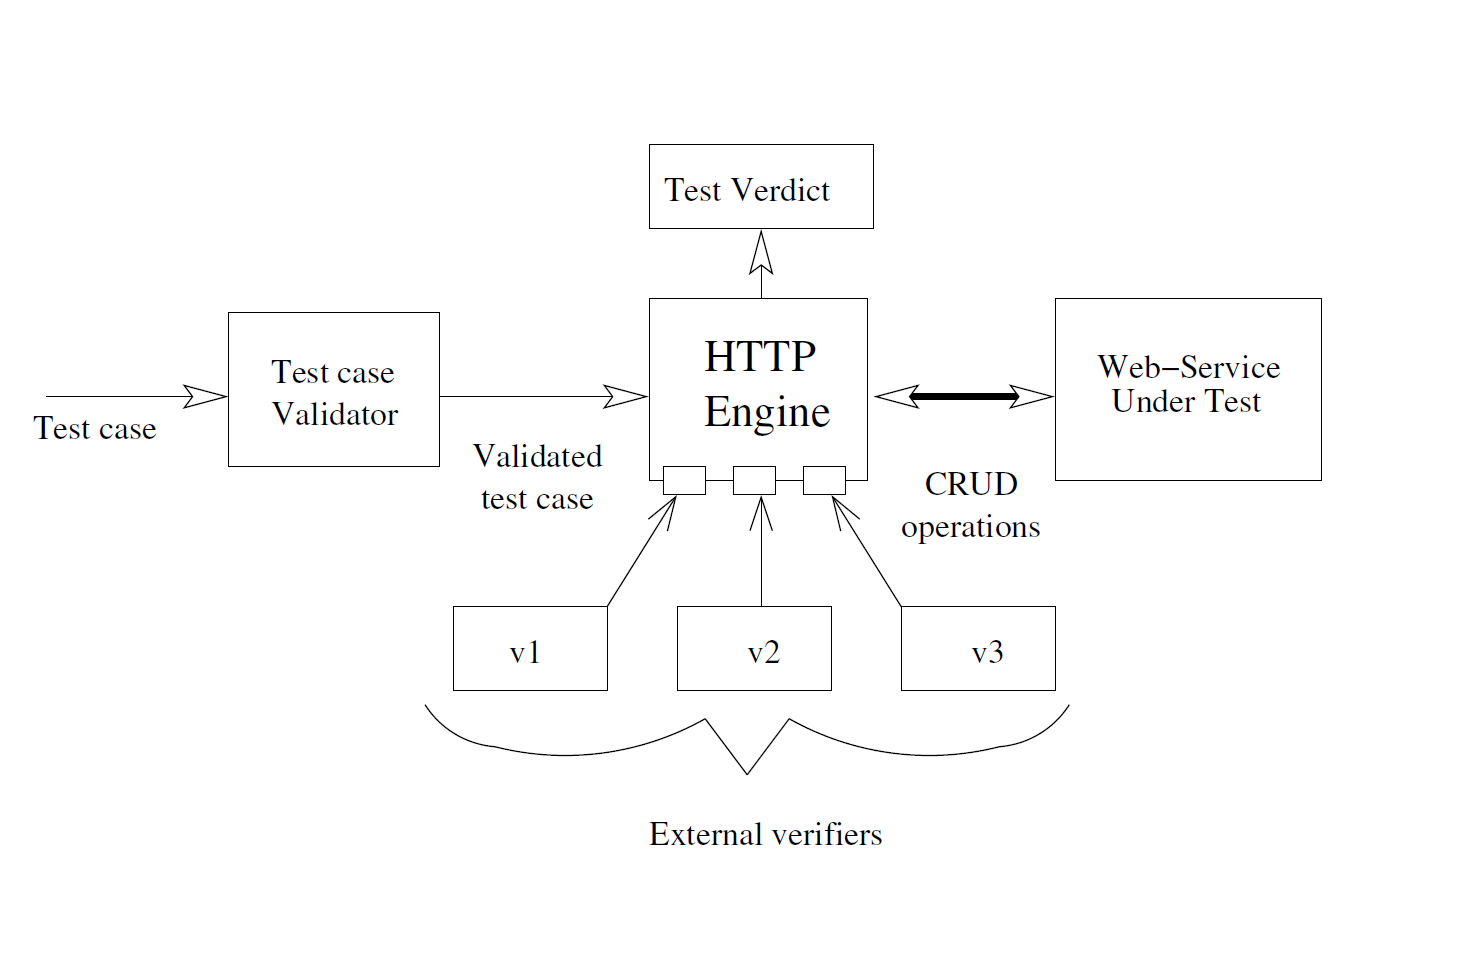
\includegraphics[width=70mm]{images/ttr_system.png}
	}
	\hfill% or \hspace{5mm} or \hspace{0.3\textwidth}
	\subfigure[Example test case]
	{
		\label{fig:ttr_test}
		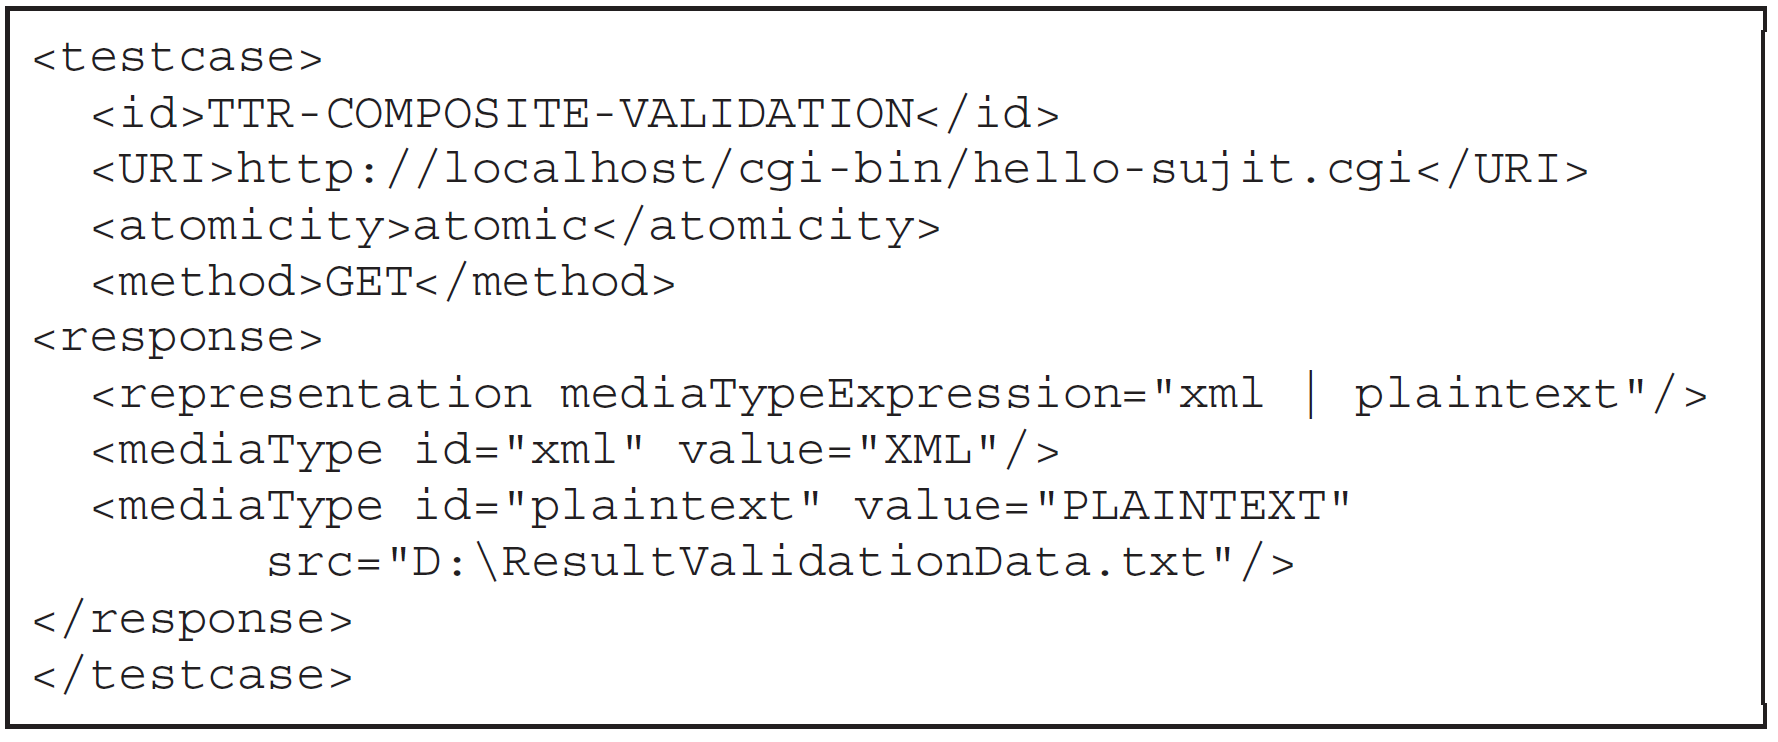
\includegraphics[width=70mm]{images/ttr_test.png}
	}
	\caption{Figure \ref{fig:ttr_system} shows the general architecture of TTR. Figure \ref{fig:ttr_test} presents an example test case written in TTR's specification language. The representation field from the response can be either XML or plain text format. Having this flexibility is particularly useful when the media-type of the response representation is not known \cite{chakrabarti2009test}.}
\end{figure}

% Second article
\textbf{Connectedness testing of RESTful web-services \cite{chakrabarti2010connectedness}.} The second article presents an algorithm to test connectedness of the RESTful web-services \cite{chakrabarti2010connectedness}. The input of the algorithm requires a specification written in WADL++ that is an extension to WADL in defining a customized format for Post Class Graphs (PCG). PCG is a visual notation to describe the problem of connectedness, it is a directed graph whose nodes represent the resources, and the edges represent the HTTP POST operation. An example PCG shown in the Figure \ref{fig:conn_poc}. WADL++ tailored for the connectedness problem in a way that it can describe which resource classes create which resource classes.

The main idea of testing connectedness is that after performing certain operations, there must be a one-to-one mapping between referenced URI list and visited URI list. If the condition meets the test passes, otherwise it fails. The overall procedure to test the connectedness of the RESTful web-service shown in the Figure \ref{fig:conn_system}. So that the approach uses PCG to generate reference URI list, and it produces related server-side resource scenario to generate visited URL list. Finally, it checks if the two outputs are equal or not.

Experiments took place in a prototype of blogging web-service called \textit{eblog}. The approach generated 16 referenced URI for comparison, and it raised exceptions for all cases in the earlier development of \textit{eblog}. Overall, the proposed tool helped in the early stage of development of \textit{eblog} to identify errors regarding broken links.
\begin{figure}[h]
	\centering
	\subfigure[]
	{
		\label{fig:conn_system}
		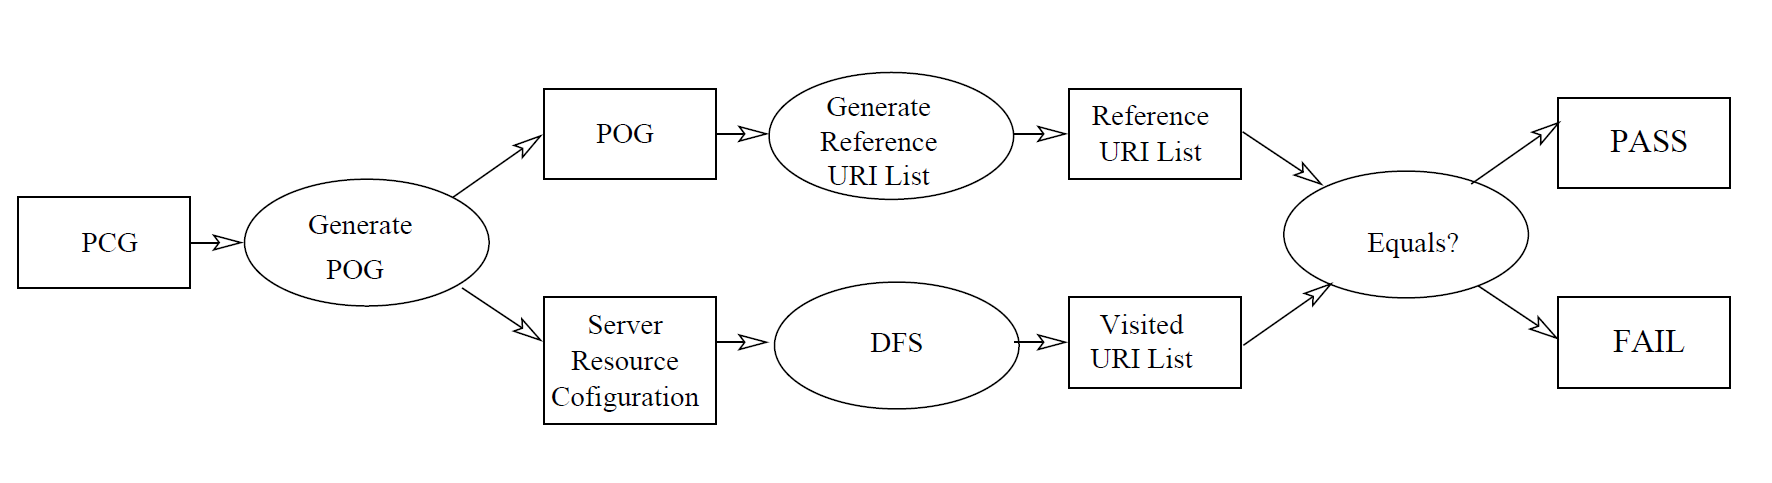
\includegraphics[width=90mm]{images/conn_system.png}
	}
	\hfill% or \hspace{5mm} or \hspace{0.3\textwidth}
	\subfigure[]
	{
		\label{fig:conn_poc}
		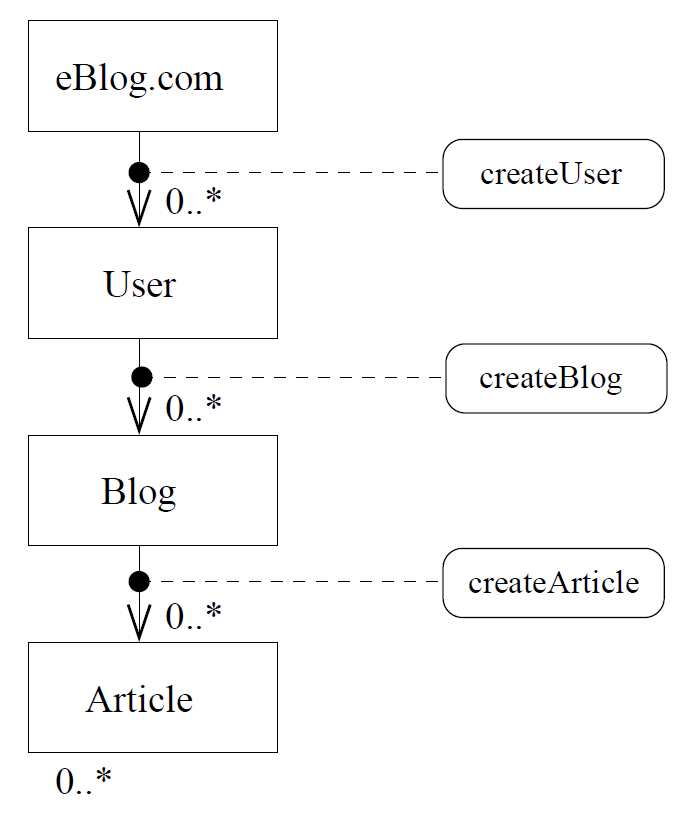
\includegraphics[width=40mm]{images/conn_poc.png}
	}
	\caption{Overall procedure of connectedness testing shown in Figure \ref{fig:conn_system}, and Figure \ref{fig:conn_poc} gives an example of Post Class Graph that belongs to prototype web-service \cite{chakrabarti2010connectedness}.}
\end{figure}

\textbf{Model-Based Testing of RESTful Web Services Using UML Protocol State Machines \cite{pinheiro2013model}.} So far we have seen that previous articles make use of specification-based testing. In this article Pinheiro et al. \cite{pinheiro2013model} presents a model-based method using UML protocol state machine to test RESTful web-services. 

The proposed system consists of many components, that is summarized by Figure \ref{fig:uml_system}. First, the tester creates the target system's behavioral model, that is protocol state machine. Then the model is converted to XML Metadata Interchange (XMI) format, which is a well-covered standard format among the modeling tools. After, each model is represented by Directed Acyclic Graph (DAG). DAG reflects only the information that belongs to system's certain states (initial, transition, and final). To generate test cases and related Java classes, the test case generation step requires test sequences and Abstract Syntactic Tree (AST) to be generated. AST is generated using expression parser from a given DAG. Furthermore, test sequences can be generated using two coverage algorithm (the tester decides which one to be used). The state coverage algorithm generates the test sequences based on DAG, whereas transition coverage algorithm based on AST. Finally, the system outputs 4 Java test classes to be able to test the system automatically.

The proposed system presents a convenient way to make model-based testing for RESTful web-services. However, no experimental evaluations about the system have been carried out.

\begin{figure}[h]
	\begin{center}
		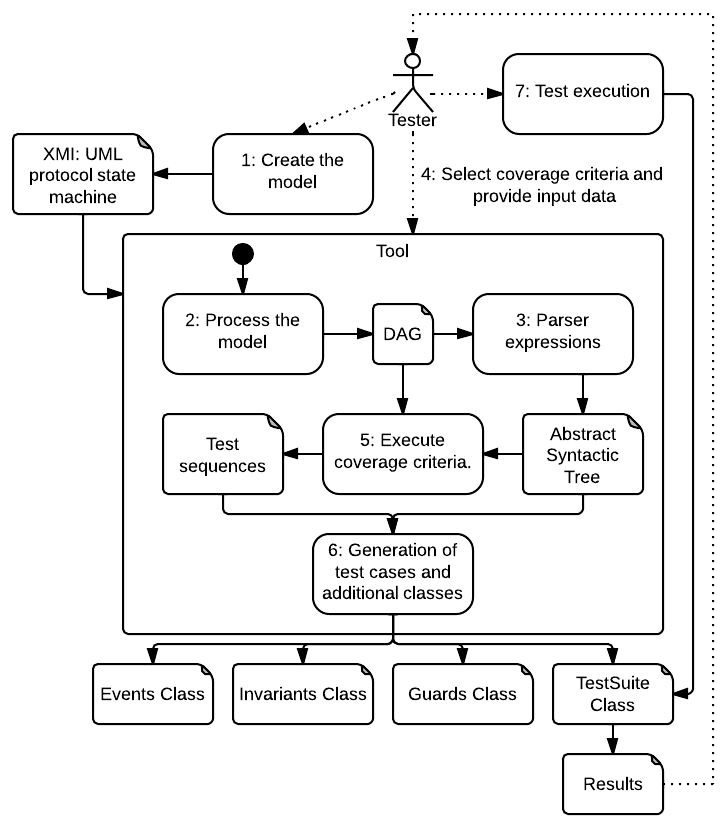
\includegraphics[width=0.45\textwidth]{images/uml_system.png}
		\caption{ Model-based RESTful web-service testing approach by Pinheiro et al. \cite{pinheiro2013model}. }
		\label{fig:uml_system}
	\end{center}
\end{figure}

\textbf{REST service testing based on inferred XML schemas \cite{navas2014rest}.} In this article Navas et al. \cite{navas2014rest} present black-box automatic error detection system for RESTful web-services based on statistical information. The method attempts to test web-services without knowing its full specification. Also, with this approach authors have opened an opportunity for this area to employ Machine Learning algorithms.

The first procedure of the system starts with a user giving an input set of test data that consists of test URL, HTTP methods, and a set of parameters for the request. Then, the REST client module reads the data and generates related REST requests to the target web-service. Each request-response pairs are stored in the database for later usage of inference module. Once the REST client tells the database location to inference module, the inferencer operates and collects the result. In the end, report generator module searches for any outliers that are obtained from the inferencer. Figure \ref{fig:xsd_system} presents the overall system architecture.

The inference module is responsible for building an XML Schema Definition (XSD) schema such that the all given documents are valid; additionally, during the process, it collects statistics about the document contents such as the number of appearances of unique elements and distribution of values for that element. It can be summarized accordingly by the given Figure \ref{fig:xsd_infer}.

Two types of experiments conducted to evaluate the system, one for the inference module, and other for the error detection system. The system is tested in Google places and configuration recovery service (their service). In the first experiment, they have compared their inference engine with existing tools Trand and SoapUI. In all cases, the inference engine surpassed the existing tools. In the second experiment no anomalies have found for Google places; however, 16 anomalies are detected for the configuration recovery service with a 56.25\% precision rate.
\begin{figure}[h]
	\centering
	\subfigure[]
	{
		\label{fig:xsd_system}
		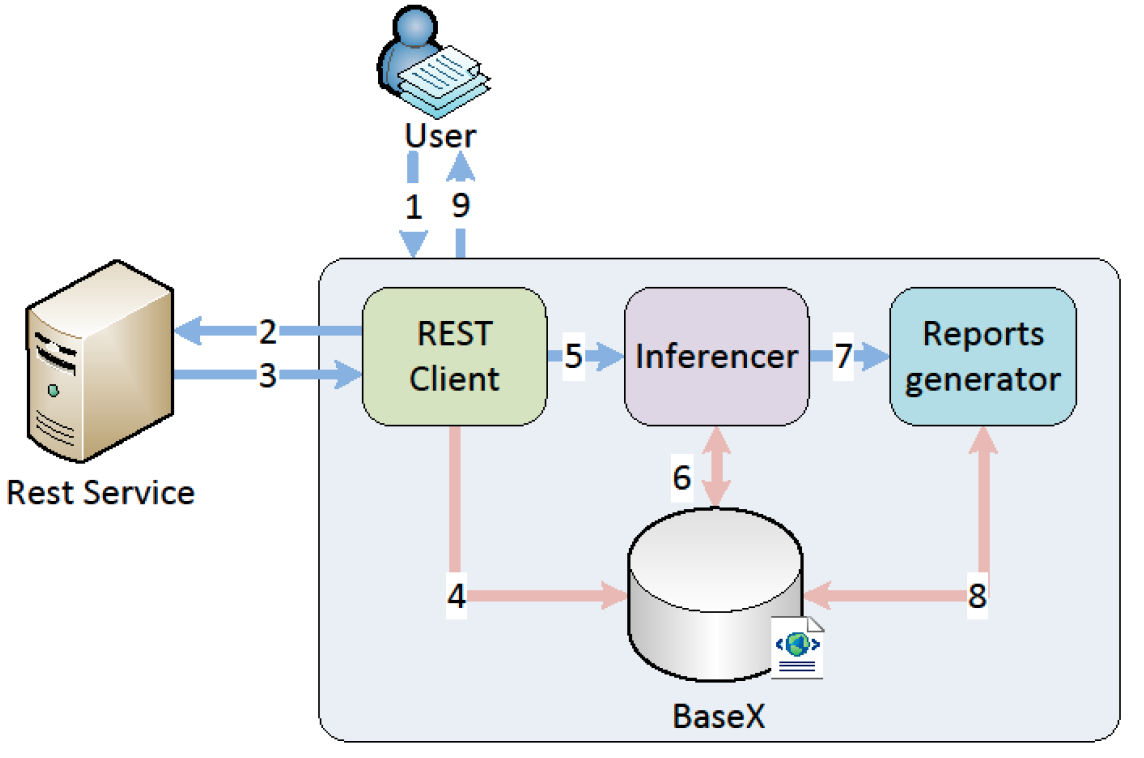
\includegraphics[width=55mm]{images/xsd_system.png}
	}
	\hfill% or \hspace{5mm} or \hspace{0.3\textwidth}
	\subfigure[]
	{
		\label{fig:xsd_infer}
		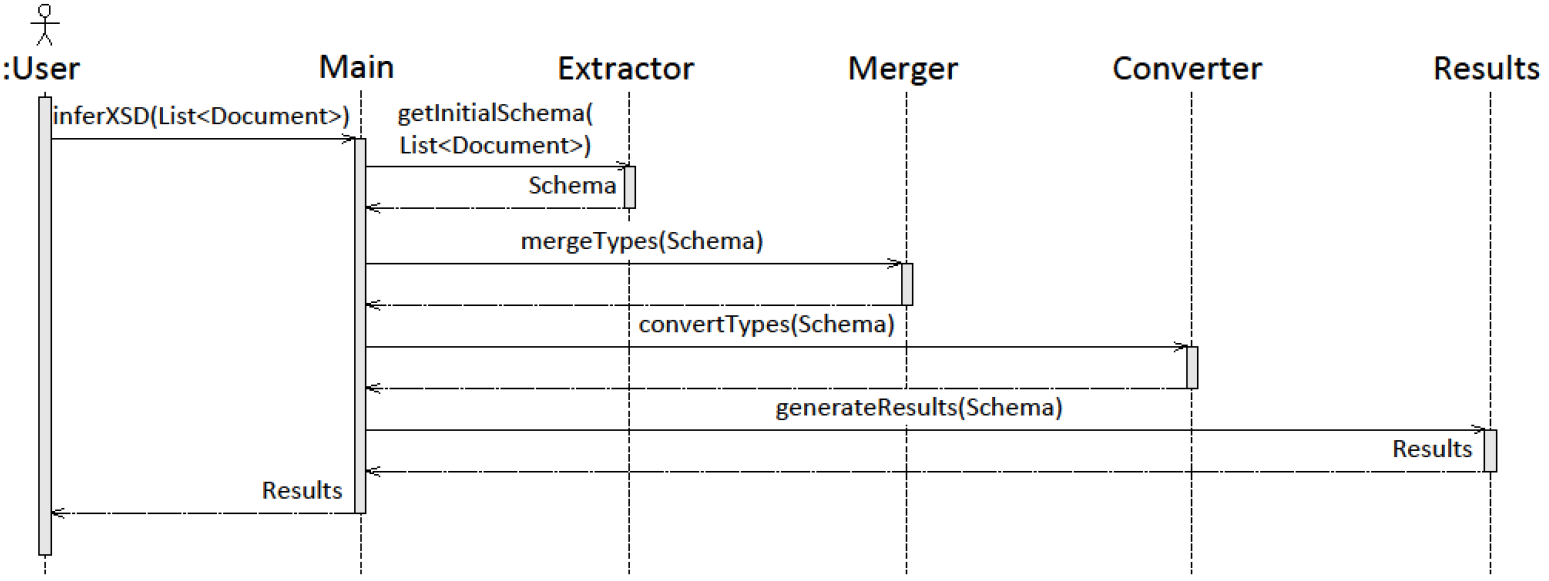
\includegraphics[width=85mm]{images/xsd_infer.png}
	}
	\caption{Figure \ref{fig:xsd_system} shows the overall system architecture, and Figure \ref{fig:xsd_infer} presents the sequence diagram of inferencer module. }
\end{figure}

\textbf{RESTful API Automated Test Case Generation \cite{arcuri2017restful}}

Paragraph to give an analysis

\subsection{System analysis}
In the literature, there are various attempts to describe and compare the different testing systems \cite{canfora2006testing, canfora2009service, bozkurt2013testing}. Since the main focus is on the different spectrum of testing approaches, neither of survey techniques in the previous articles are not directly feasible for our document. Besides, we believe that it does not give enough detail concerning practical implications. Given the fact, comparative analysis of the five RESTful web-service testing methods is focused on mainly to following criterion: methodology, practicality, and evaluation.

Methodology comparisons and critics.

Practicality comparisons and critics.

Evaluation comparisons and critics.

Explanation of the table.

\begin{table}[h]
	\begin{center}
		\hspace*{-1.25cm}
		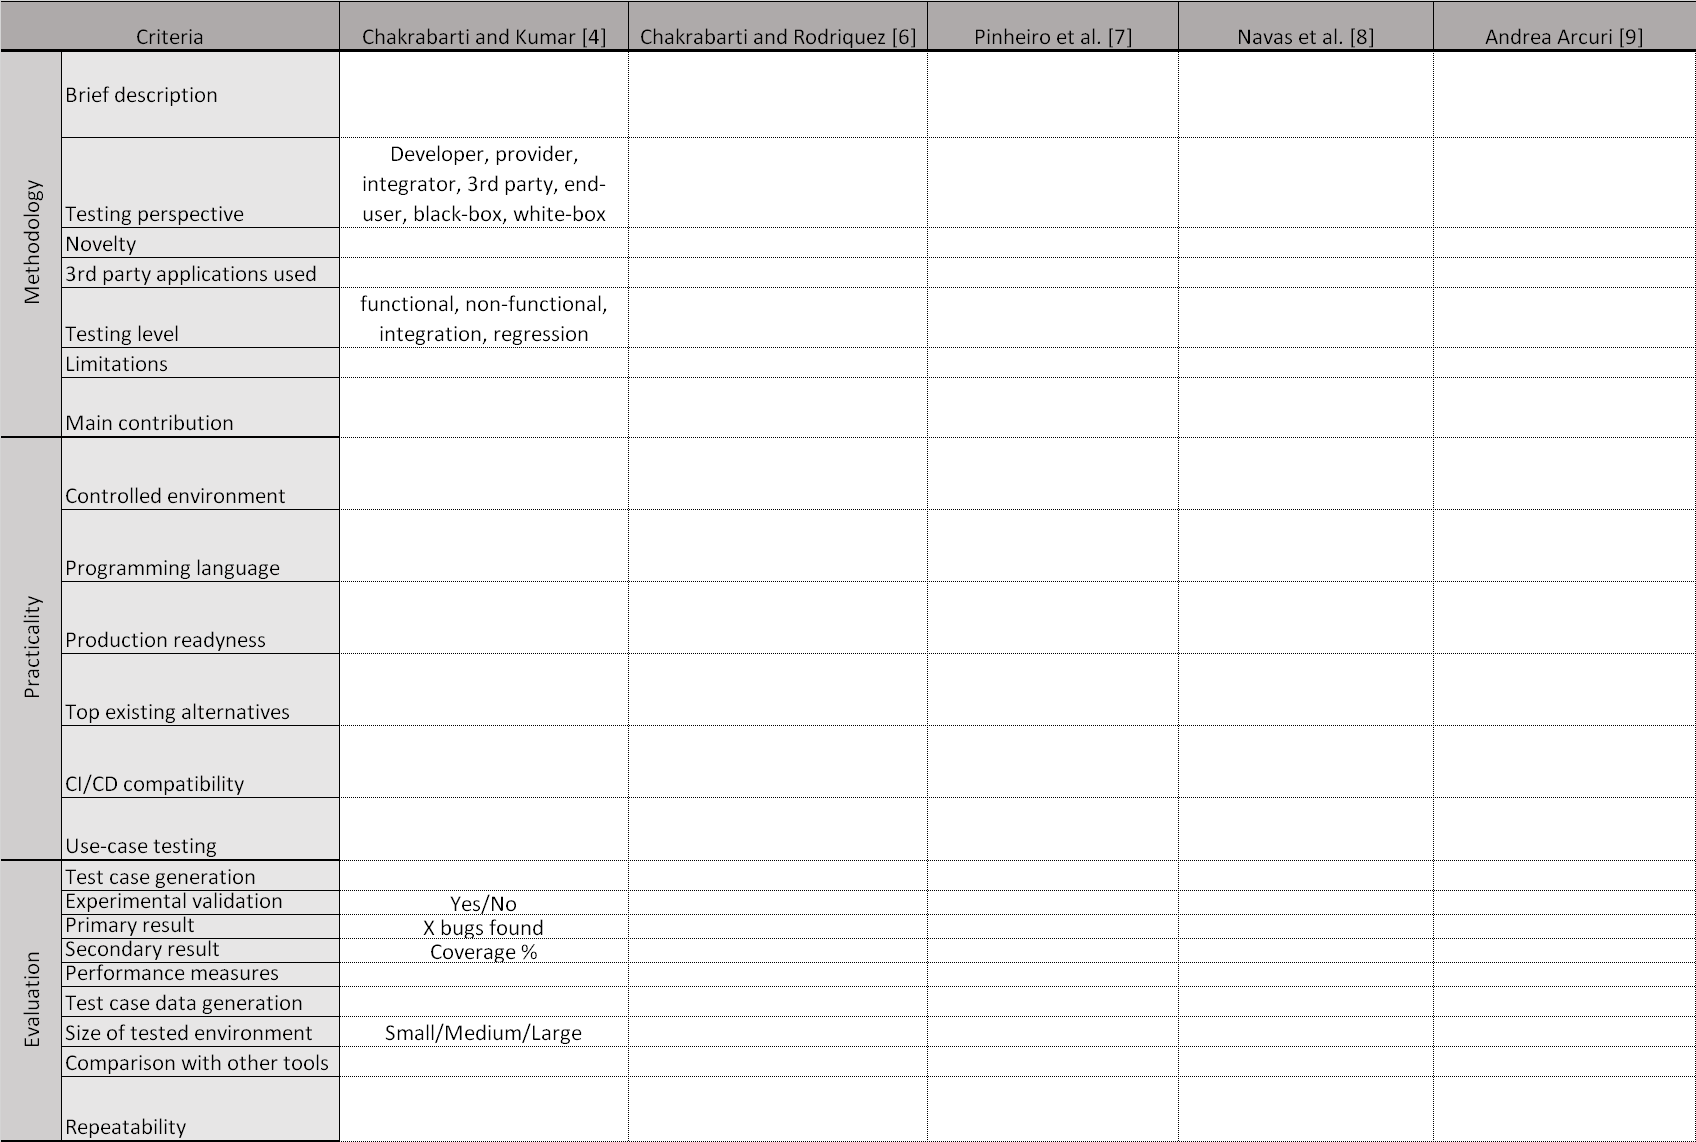
\includegraphics[width=1.1\textwidth]{images/comparison.png}
		\caption{The comparison matrix presents ...}
		\label{table:comparison}
	\end{center}
\end{table}

\section{Future research}
Talk about machine learning, search-based algorithms, evolutionary algorithms.

Production ready approaches = NO

Validation of approaches in the experiments. 

\section{Conclusion}
Present the topic again, summarize, and conclude with a future tendency under the consideration of testing the rest.

\newpage
\nocite{*}
% one of these or  ...
%\bibliographystyle{plain}
%\bibliographystyle{acm}
\bibliographystyle{ieeetr}

% ... or this 
%\bibliographystyle{apalike}

\bibliography{references}

\lastpage

\end{document}